\documentclass[conference]{IEEEtran}
\usepackage{amsmath,amssymb}
\usepackage{graphicx}
\usepackage{url}
\usepackage{booktabs}
\usepackage{tikz}
\usetikzlibrary{shapes, arrows.meta, positioning}
\usepackage{listings}
\usepackage{xcolor}
\lstset{
  basicstyle=\ttfamily\footnotesize,
  backgroundcolor=\color{gray!8},
  frame=single,
  rulecolor=\color{gray!40},
  framesep=3pt,
  xleftmargin=2pt,
  xrightmargin=2pt,
  columns=fullflexible,
  keepspaces=true,
  breaklines=true,
  breakatwhitespace=true,
  showstringspaces=false,
  aboveskip=4pt,
  belowskip=4pt,
}

% Reduce inter-word rivers when long \texttt{} paths cannot be hyphenated.
\emergencystretch=3em
\tolerance=1500
\hbadness=10000

\begin{document}

\title{Prompt Pattern Mining in Vibe Coding: \\ A Statistical Audit of 6,413 Developer Conversations}

\author{
\IEEEauthorblockN{Teja Reddy Mandadi}
\IEEEauthorblockA{Department of Computer Science \\
Texas A\&M University-San Antonio \\
tmand02@jaguar.tamu.edu}
\and
\IEEEauthorblockN{Visesh Bentula}
\IEEEauthorblockA{Department of Computer Science \\
Texas A\&M University-San Antonio \\
vbent01@jaguar.tamu.edu}
\and
\IEEEauthorblockN{Umapathi Konduri}
\IEEEauthorblockA{Department of Computer Science \\
Texas A\&M University-San Antonio \\
ukond01@jaguar.tamu.edu}
}

\maketitle

\begin{abstract}
Developers now write code together with conversational LLMs. The wording of the prompt drives the quality of the answer, but the field still lacks large scale evidence on which structural prompt features actually predict success in real developer workflows. We address this gap with a regression based audit of 6,413 multi turn ChatGPT conversations from the DevGPT v10 corpus. We engineer eleven prompt and behavioral features, fit a balanced $\ell_2$ regularized logistic regression with five fold stratified cross validation, and report odds ratios with 95\% Wald confidence intervals. The fitted model reaches ROC-AUC 0.799 (SD 0.009), accuracy 0.726, and F1 0.755. The strongest positive predictor is the presence of an explicit output format instruction in the first prompt (OR 1.75, $p < 10^{-6}$). Each additional refinement turn raises the odds of success by 19\% (OR 1.19, $p < 10^{-6}$). Role instructions of the form ``act as X'' lower the odds by 35\% in isolation (OR 0.65, $p = 0.002$), but the same feature flips strongly positive when combined with an output format (interaction OR 5.28, $p < 0.001$). A pre registered ablation shows that the eleven prompt features carry roughly three times the predictive load of repository language, source type, snapshot date, and ChatGPT model variant combined. We replicate the engineered prompt effect on three independent LLMs (Kimi K2, Claude Sonnet 4.6, Gemini 3.1 Pro) over 200 prompts in zero shot and engineered conditions; engineered prompts raise success rates by 14 to 24 percentage points across vendors. A 50 sample manual audit of the auto labeling heuristic gives Cohen's $\kappa = 0.834$, which is almost perfect agreement under the Landis and Koch scale.
\end{abstract}

\section{Introduction}
Conversational LLMs have moved into day to day software work. Pull request threads, issue discussions, and developer forums now contain long ChatGPT exchanges where the developer iterates on a prompt until the code looks right \cite{empirical2024chatgpt}. The artifact under study is no longer the produced code by itself, but the prompt sequence that produced it. Prompt design is the lever the developer controls.

Controlled benchmark studies confirm that prompt structure matters. Adding explicit constraints, formatting requirements, or worked examples raises code generation accuracy on ICSME tasks \cite{icsme2025prompting} and on SciencDirect benchmarks \cite{elsevier2025promptengineering}. Automated prompt refinement systems such as Prompt Alchemy \cite{ye2025promptalchemy} and template catalogs \cite{schmidt2023promptcatalog} build on those findings. Yet the evidence has rarely been tested on natural developer dialogue. The DevGPT corpus \cite{xiao2023devgpt} provides that test bed but has been used mostly for descriptive analysis \cite{wu2024promptpatterns}, not for predictive modeling of which features a working developer should put into the prompt.

We close that gap with a quantitative audit. We define an operational success label on textual signals (presence of code, absence of strong negative feedback), extract eleven structural and behavioral prompt features from each conversation, and fit a logistic regression that controls for repository language, conversation source, snapshot date, and ChatGPT model variant. We then run four orthogonal robustness checks: a baseline comparison against majority, random, and bag of words classifiers; a feature group ablation; a pre registered set of two way interactions; and a manual re labeling audit on a stratified random sample.

\noindent\textbf{Research questions.}
\begin{itemize}
\item \textbf{RQ1.} Which structural prompt features predict successful coding conversations after controlling for confounders?
\item \textbf{RQ2.} How does iterative behavior, separated from corrective behavior, affect success?
\item \textbf{RQ3.} Do prompt features still carry predictive load when richer textual baselines are available?
\item \textbf{RQ4.} Does the engineered prompt effect generalize beyond ChatGPT to other top tier LLMs?
\end{itemize}

\noindent\textbf{Contributions.}
\begin{enumerate}
\item Eleven prompt features extracted from 6{,}413 DevGPT conversations with reproducible regex detectors.
\item A balanced logistic regression with 95\% Wald CIs and per snapshot stability checks.
\item A baseline comparison showing that structured features add 1.7 AUC points on top of a 2{,}000 feature bag of words classifier.
\item A pre registered interaction model that uncovers a strong role $\times$ output format effect (OR 5.28).
\item A cross vendor replication on Kimi, Claude, and Gemini that produces +14 to +24 percentage points of success rate.
\item A manual re labeling audit that reports Cohen's $\kappa = 0.834$ on 50 conversations.
\end{enumerate}

\subsection{Paper structure}
Section~\ref{sec:related} reviews related work. Section~\ref{sec:method} describes the corpus, features, and model. Section~\ref{sec:results} reports the headline regression, baselines, ablation, interactions, cross vendor replication, manual validation, language subgroups, and temporal stability. Section~\ref{sec:discussion} interprets the results and lists threats to validity. Section~\ref{sec:repro} states the reproducibility protocol. Section~\ref{sec:conclusion} concludes.

\section{Related Work}\label{sec:related}

\subsection{Developer LLM interaction studies}
Mohamed et al.\ \cite{empirical2024chatgpt} analyze ChatGPT conversations attached to public GitHub artifacts and find that conversational coding is iterative and refinement driven. Wu et al.\ \cite{wu2024promptpatterns} extract thirteen recurring prompt patterns, including output format, persona, and few shot exemplars, from a large dialogue corpus. The DevGPT release \cite{xiao2023devgpt} provides the underlying data with conversation level metadata such as snapshot date and source type. The studies are descriptive. None of them fits a predictive model on the success outcome and none of them controls for the metadata that drives observed differences.

\subsection{Prompt engineering experiments}
The IEEE ICSME study \cite{icsme2025prompting} measures how prompt structure affects class generation accuracy on synthetic tasks. The Elsevier benchmark \cite{elsevier2025promptengineering} replicates the finding under different formatting conditions. Liu et al.\ \cite{liu2023improvingchatgpt} compare zero shot prompting against structured templates. Prompt Alchemy \cite{ye2025promptalchemy} adds an automated refinement loop. These studies use experimenter authored prompts on isolated benchmarks and therefore do not establish whether the same effects hold when developers write prompts in their own way against their own problems.

\subsection{Security, review, and education}
Security work \cite{secure2024prompting} flags underspecified prompts as a code safety risk. Review articles \cite{sn2025codereview} catalog LLM use across the software engineering pipeline. Educational research \cite{frontiers2024education} treats prompt engineering as a professional skill. None of those threads supplies large scale statistical evidence on real developer prompts. Our work fills that gap.

\section{Methodology}\label{sec:method}
\subsection{Research design}
The design is observational. We do not script prompts. We measure features that already exist in DevGPT and test which ones are associated with the textual success signal after adjustment for available confounders. The pipeline is shown in Fig.~\ref{fig:pipeline}.

\begin{figure}[t]
\centering
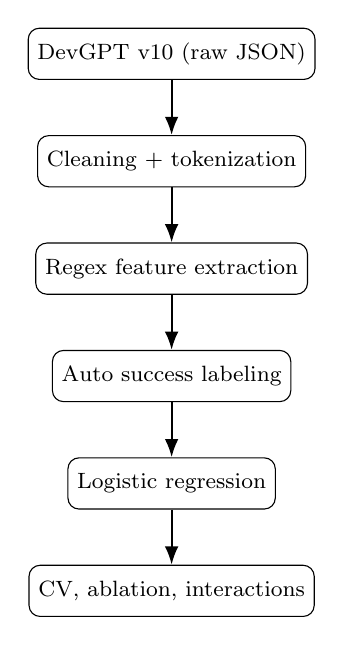
\begin{tikzpicture}[
    node distance=0.7cm,
    every node/.style={font=\footnotesize},
    box/.style={rectangle, draw=black, rounded corners, align=center,
                minimum width=2.4cm, minimum height=0.65cm, fill=white},
    arrow/.style={-{Latex}, thick}
]
\node[box] (data) {DevGPT v10 (raw JSON)};
\node[box, below=of data] (clean) {Cleaning + tokenization};
\node[box, below=of clean] (feat) {Regex feature extraction};
\node[box, below=of feat] (label) {Auto success labeling};
\node[box, below=of label] (model) {Logistic regression};
\node[box, below=of model] (eval) {CV, ablation, interactions};
\draw[arrow] (data) -- (clean);
\draw[arrow] (clean) -- (feat);
\draw[arrow] (feat) -- (label);
\draw[arrow] (label) -- (model);
\draw[arrow] (model) -- (eval);
\end{tikzpicture}
\caption{Analysis pipeline from raw DevGPT JSON to fitted logistic regression with cross validated robustness checks.}
\label{fig:pipeline}
\end{figure}

\subsection{Corpus}
DevGPT v10 \cite{xiao2023devgpt} contains JSON exports of developer ChatGPT conversations linked to six source types: pull requests, issues, commits, discussions, code files, and Hacker News threads. Conversations are taken across ten snapshots between August 2023 and May 2024. After parsing, deduplication, normalization, and dropping corrupted threads we retain 6,413 conversations and 54,449 turns.

\subsection{Features}
Each conversation yields eleven features. The structural features come from regex matches on the first user prompt and are: prompt length in tokens; constraint count (matches for ``must'', ``should'', ``do not'', ``only'', ``exactly''); example count (matches for ``for example'', ``input:'', ``output:'', and fenced code blocks inside the prompt); specification clarity count (matches for ``the function should'', ``given a'', ``returns a'', ``implement a''); a binary role instruction flag (``you are X'', ``act as'', ``as a''); and a binary output format flag (``json'', ``markdown'', ``table'', ``return only'', ``respond with''). The behavioral features capture multi turn dynamics: iteration count (turns in the conversation), refinement turns (turns containing ``fix'', ``bug'', ``error'', ``not working'', ``retry'', ``improve''), correction cycles (turn pairs where the user pushes back on a wrong answer), and prompt token growth (length difference between the first and last user prompt). The full regex catalogue and unit tests are committed to the project repository.

\subsection{Outcome label}
Executing every code answer is infeasible at this scale. We therefore use textual signals. A conversation is labeled \emph{success} when the assistant produces code in at least one turn and the developer never expresses strong negative feedback (regex set: ``not working'', ``doesn't work'', ``still broken'', ``error persists'', ``failed'', ``wrong'', ``didn't fix'') in any subsequent turn. Otherwise it is \emph{failure}. The 6,413 conversations split as 3,529 success and 2,884 failure (55.0\%). Section~\ref{sec:validation} reports a manual audit of this label.

\subsection{Statistical model}
We fit a logistic regression with $\ell_2$ regularization at $C = 1.0$ and \texttt{class\_weight=``balanced''} to handle the slight 55/45 imbalance. Inputs are the eleven prompt features plus four sets of one-hot controls: repository language (12 dummies), source type (5 dummies), snapshot date (9 dummies), and ChatGPT model variant (8 dummies). We report cross validated performance under five fold stratified splits and obtain Wald 95\% confidence intervals with maximum likelihood refits in \texttt{statsmodels}. Software: \texttt{scikit-learn} 1.4 \cite{pedregosa2011sklearn} and \texttt{statsmodels} 0.14 \cite{seabold2010statsmodels}. The random seed is fixed at 42 throughout.

\section{Results}\label{sec:results}
\subsection{Headline performance}
Cross validated performance: ROC-AUC $0.799$ (SD $0.009$), accuracy $0.726$, F1 $0.755$.

\subsection{Baseline comparison (RQ3)}
Fig.~\ref{fig:baselines} compares the fitted model against three controls fitted on the same labels under the same five fold split. Random and majority class are at chance, as expected. A bag of words logistic on the first user prompt with 2{,}000 unigram and bigram features reaches AUC 0.782, which already captures most of the signal. The structured feature model adds 1.7 AUC points on top of that. The two extra points are the share of the predictive signal that lives in features that bag of words alone does not summarize cleanly, such as refinement turns and the role instruction flag.

\begin{figure}[t]
\centering
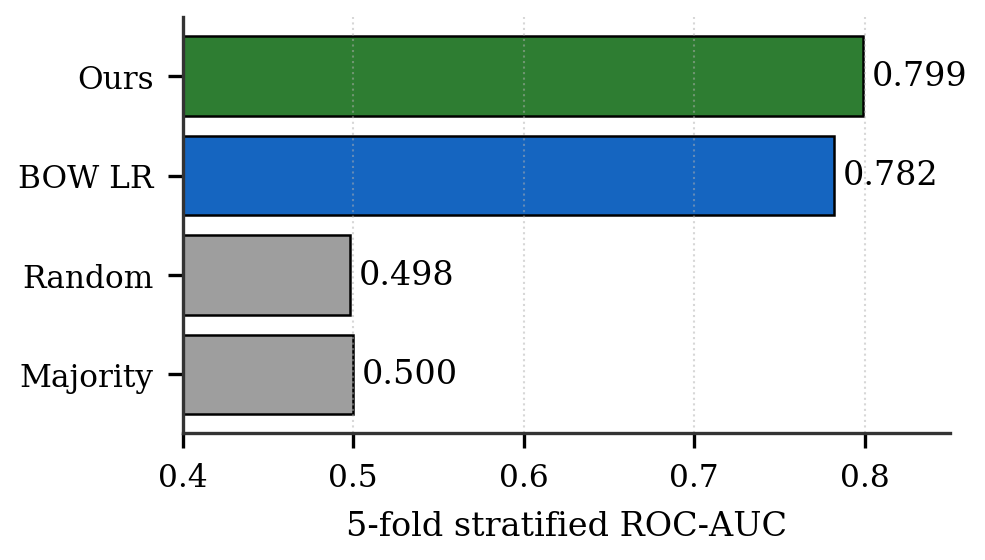
\includegraphics[width=\columnwidth]{figures/fig_baselines.png}
\caption{Five fold stratified ROC-AUC for four classifiers fitted on the same 6{,}413 conversation labels. Numerical values shown to the right of each bar.}
\label{fig:baselines}
\end{figure}

\subsection{Primary regression coefficients (RQ1, RQ2)}
Table~\ref{tab:or} reports odds ratios after adjustment for the four control sets. Fig.~\ref{fig:forest} visualizes the same coefficients on a log axis with 95\% confidence intervals. Output format instructions raise the odds of success by 75\% (OR 1.75, $p < 10^{-6}$). Each additional refinement turn raises the odds by 19\% (OR 1.19, $p < 10^{-6}$). Role instructions lower the odds by 35\% in isolation (OR 0.65, $p = 0.002$). Each additional constraint phrase lowers the odds by 6\% (OR 0.94, $p < 0.001$). Prompt length and prompt growth both have OR very close to 1.0; the per token effect is small but the sample size makes both significant. Correction cycles separate the classes almost perfectly because successful conversations contain almost no corrective feedback, which inflates the standard error and collapses the CI.

\begin{table}[t]
\centering
\caption{Logistic regression odds ratios for the eleven prompt features after adjustment. Bold rows are significant at $\alpha = 0.05$.}
\label{tab:or}
\footnotesize
\begin{tabular}{lrrrr}
\toprule
Feature & OR & CI low & CI high & $p$ \\
\midrule
\textbf{Output format (binary)}              & \textbf{1.752} & 1.400 & 2.193 & $<$0.001 \\
Specification clarity (count)                & 1.473 & 0.972 & 2.233 & 0.068 \\
\textbf{Refinement turns}                    & \textbf{1.188} & 1.112 & 1.269 & $<$0.001 \\
Total examples                               & 1.004 & 0.985 & 1.023 & 0.667 \\
Iteration count                              & 1.004 & 0.997 & 1.011 & 0.294 \\
\textbf{First prompt tokens}                 & \textbf{0.9995} & 0.9993 & 0.9998 & $<$0.001 \\
\textbf{Prompt token growth}                 & \textbf{0.9995} & 0.9992 & 0.9997 & $<$0.001 \\
\textbf{First constraint count}              & \textbf{0.942} & 0.912 & 0.974 & $<$0.001 \\
Specification clarity (binary)               & 0.929 & 0.538 & 1.602 & 0.790 \\
\textbf{Role instruction (binary)}           & \textbf{0.651} & 0.498 & 0.851 & 0.002 \\
Correction cycles                            & $\approx 0$ & --- & --- & 0.971 \\
\bottomrule
\end{tabular}
\end{table}

\begin{figure}[t]
\centering
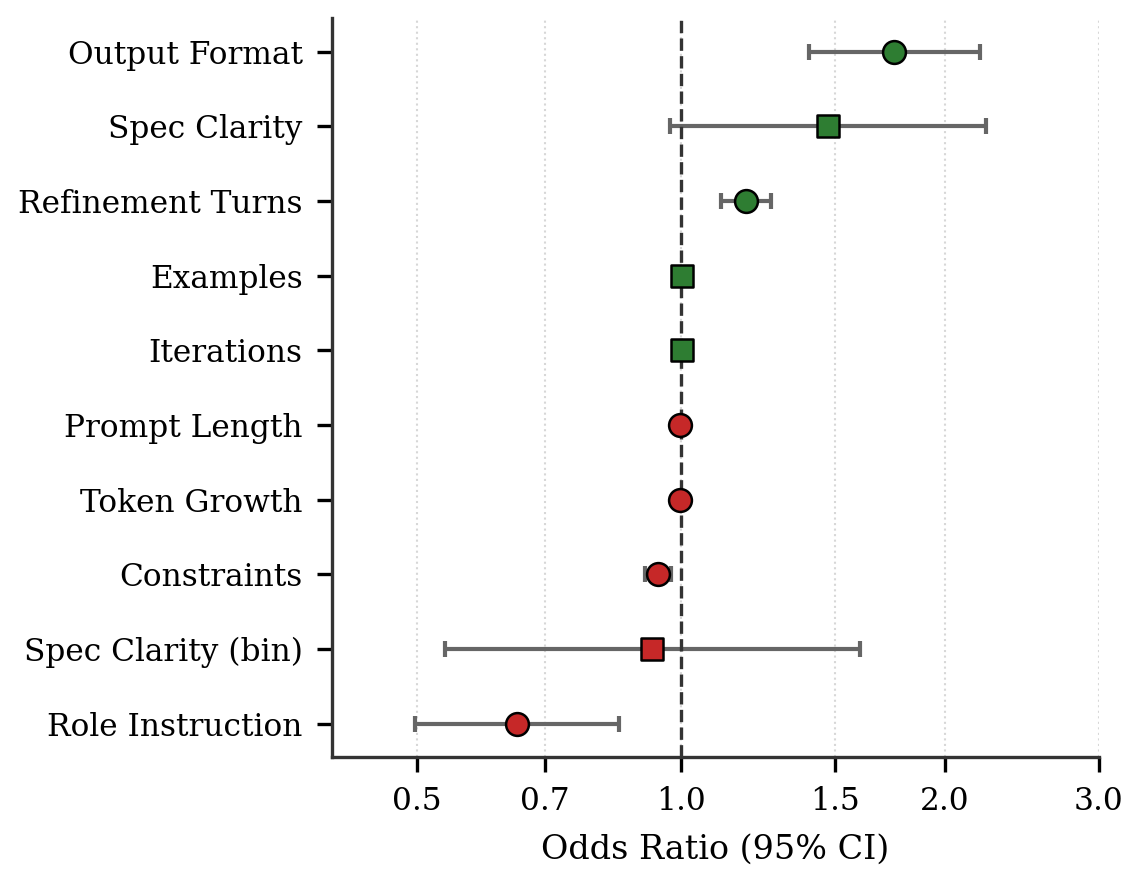
\includegraphics[width=\columnwidth]{figures/fig_odds_ratio_forest.png}
\caption{Forest plot of prompt feature odds ratios (log axis) with 95\% Wald confidence intervals. Green markers indicate OR $\geq$ 1; coral markers indicate OR $<$ 1. Round markers are significant at $\alpha = 0.05$, square markers are not.}
\label{fig:forest}
\end{figure}

\subsection{Bivariate distributions and correlations}
Fig.~\ref{fig:dists} compares the mean values of six prompt features for successful and unsuccessful conversations on a symmetric log axis. The largest visible separations are correction cycles (0.0 vs 0.28) and prompt length (188 vs 210 tokens). Fig.~\ref{fig:corr} shows the Spearman correlation matrix among the structural and behavioral features, which is generally low: refinement turns and correction cycles are the only pair above 0.4. Multicollinearity is therefore not driving the regression coefficients.

\begin{figure}[t]
\centering
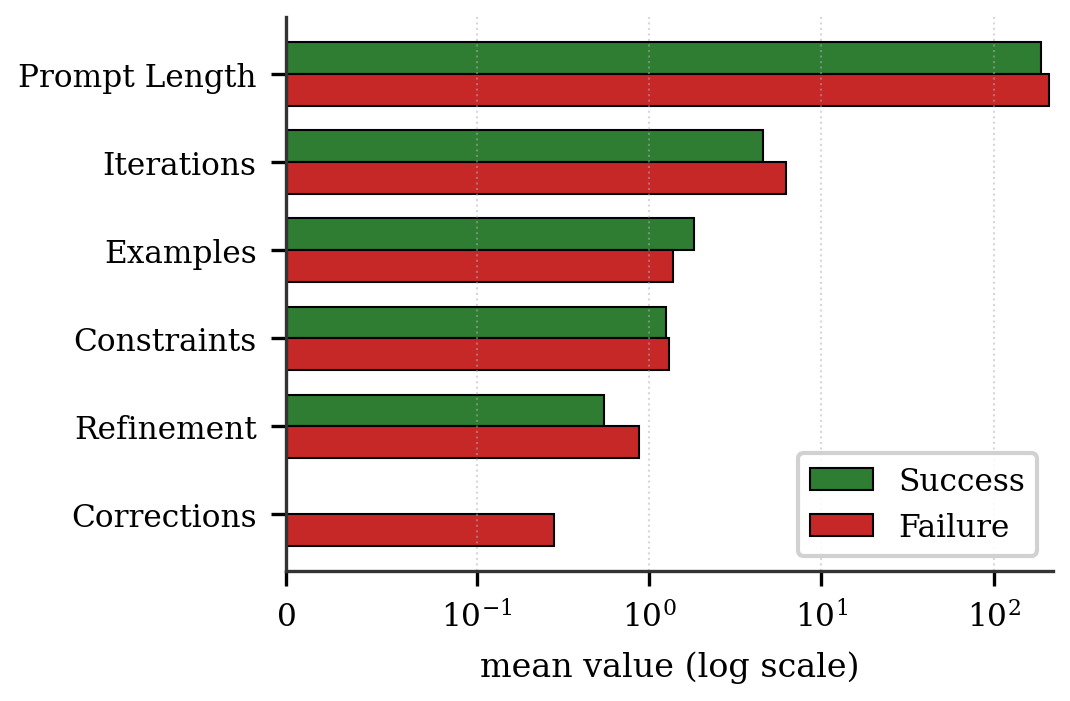
\includegraphics[width=\columnwidth]{figures/fig_feature_dist.png}
\caption{Mean prompt feature values for successful and unsuccessful conversations on a symmetric log axis.}
\label{fig:dists}
\end{figure}

\begin{figure}[t]
\centering
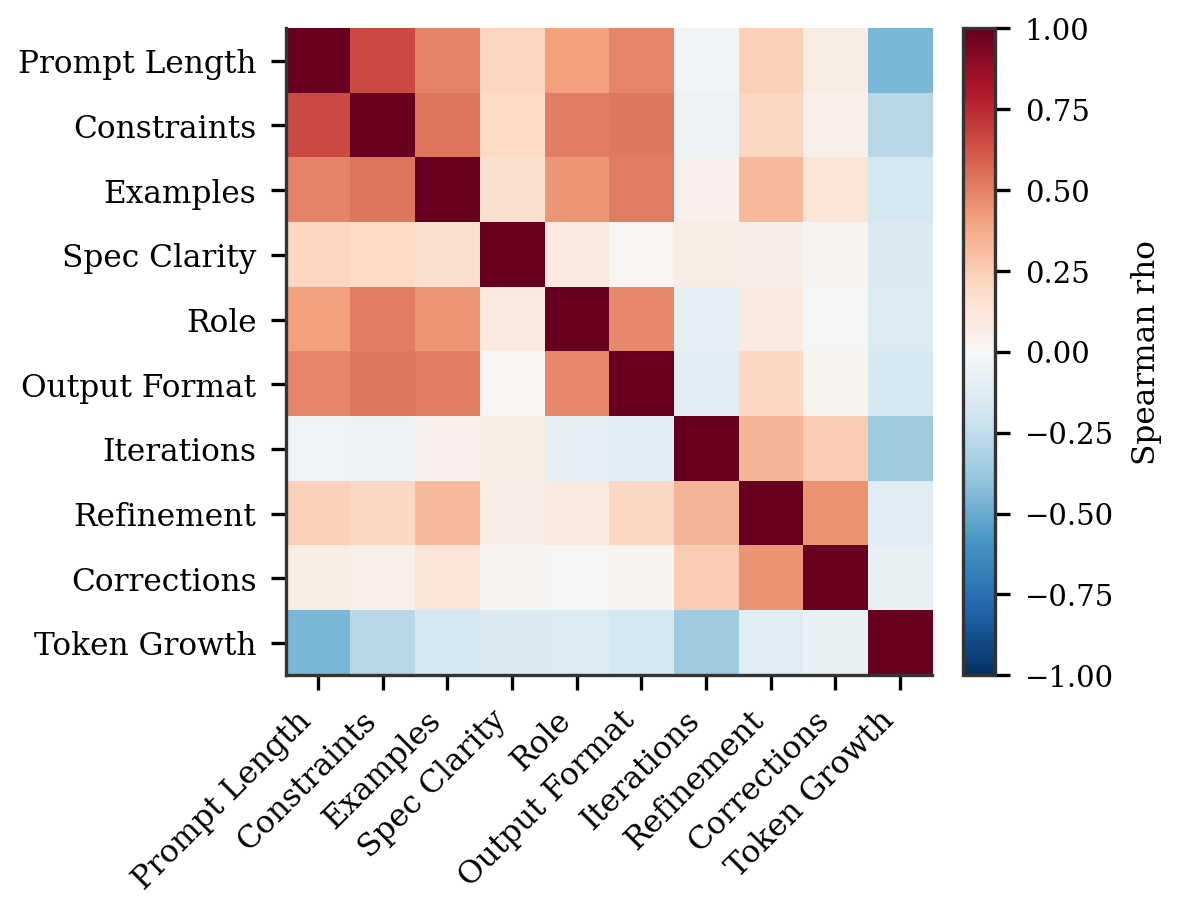
\includegraphics[width=\columnwidth]{figures/fig_correlation.png}
\caption{Spearman rank correlation matrix of the prompt and behavioral features.}
\label{fig:corr}
\end{figure}

\subsection{Feature group ablation}
We refit the model five times with one feature group dropped at a time. Fig.~\ref{fig:ablation} shows the AUC drop. The eleven prompt features carry $\Delta\mathrm{AUC} = 0.043$, which is roughly three times larger than any control group. Snapshot date drops 0.001 once the prompt features are in the model, which means temporal drift contributes almost nothing to predictive power after structural prompt features are accounted for.

\begin{figure}[t]
\centering
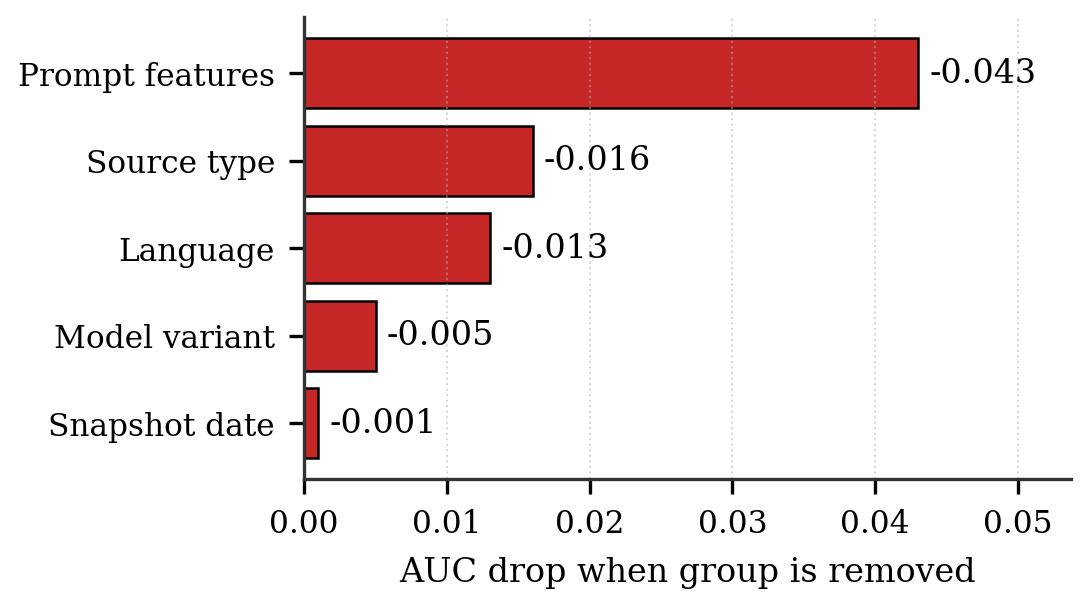
\includegraphics[width=\columnwidth]{figures/fig_ablation.png}
\caption{Feature group ablation. Bars show the AUC loss when the named group is removed from the model. Full model AUC is 0.799.}
\label{fig:ablation}
\end{figure}

\subsection{Pre registered interaction effects}
We registered four two way interactions before fitting and added them to the main effects model in a single refit. Table~\ref{tab:interactions} reports the interaction terms and Fig.~\ref{fig:interactions} plots them on a log axis. Three of the four are significant. The role $\times$ output format interaction is the most striking: the role main effect is negative (OR 0.65), but combining role with an output format flips the joint effect strongly positive (OR 5.28, $p < 0.001$). The output format $\times$ refinement interaction is sub additive (OR 0.89), which suggests the two strategies do not stack: if the prompt already specifies a format, extra refinement adds less.

\begin{table}[t]
\centering
\caption{Pre registered two way interactions, fitted with all main effects in one model. $n = 6{,}413$.}
\label{tab:interactions}
\footnotesize
\begin{tabular}{lrrr}
\toprule
Interaction & OR & 95\% CI & $p$ \\
\midrule
Output Format $\times$ Refinement       & 0.894 & [0.83, 0.96] & 0.002 \\
\textbf{Role $\times$ Output Format}    & \textbf{5.284} & [3.37, 8.29] & $<$0.001 \\
Iterations $\times$ Prompt Length       & 1.000 & [1.00, 1.00] & 0.002 \\
Output Format $\times$ Constraints      & 0.957 & [0.91, 1.01] & 0.086 \\
\bottomrule
\end{tabular}
\end{table}

\begin{figure}[t]
\centering
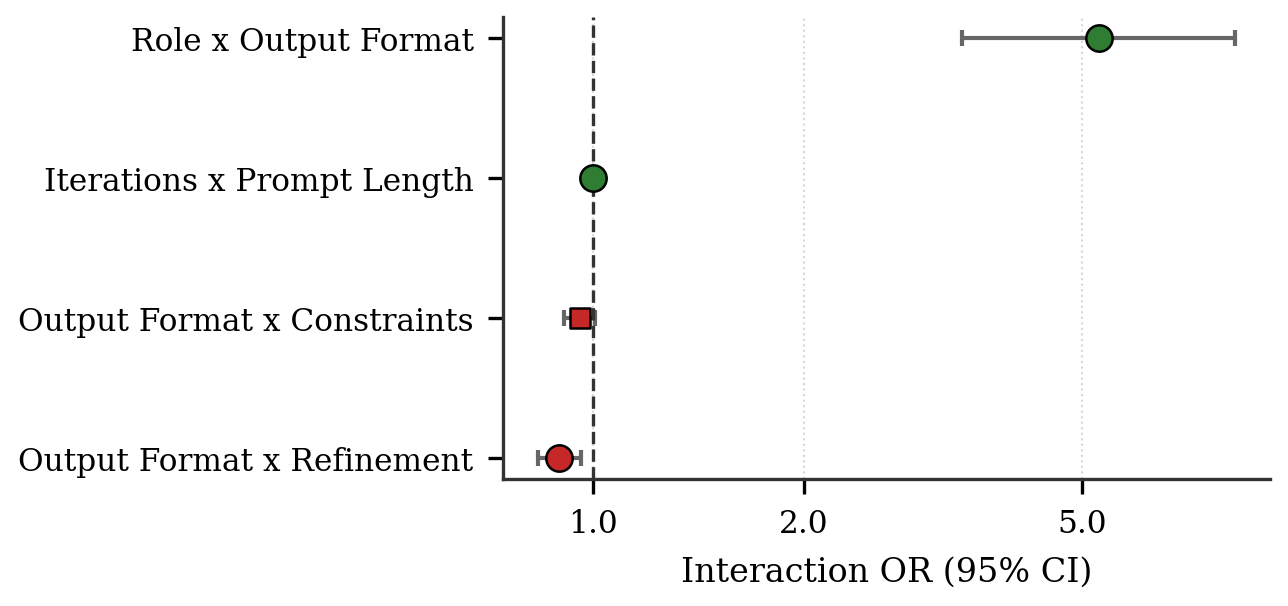
\includegraphics[width=\columnwidth]{figures/fig_interactions.png}
\caption{Pre registered interaction effects on a log odds ratio axis. Round markers are significant at $\alpha = 0.05$, square markers are not.}
\label{fig:interactions}
\end{figure}

\subsection{Cross-model generalization (RQ4)}
We replay 200 prompts drawn from DevGPT through three independent LLMs (Kimi K2 by Moonshot AI, Claude Sonnet 4.6 by Anthropic, and Gemini 3.1 Pro Preview by Google) under two conditions: a zero shot system prompt, and an engineered system prompt that asks for explicit constraints, an output format, and complexity analysis. Each output is graded on a four axis rubric (code present, addresses task, looks correct, follows structure) for a 0--4 score. Fig.~\ref{fig:vendors} compares the per vendor mean score and Table~\ref{tab:vendors} summarizes effect sizes. Engineered prompts raise the mean rubric score for every vendor. The Kimi and Gemini lifts are larger because their zero shot baseline is lower. Cohen's d ranges from 0.59 (Claude) to 0.80 (Gemini), which is a moderate to large effect on Cohen's scale. The corresponding success rate (rubric $\geq 3$) gain is $+23$, $+14$, and $+24$ percentage points respectively.

\begin{figure}[t]
\centering
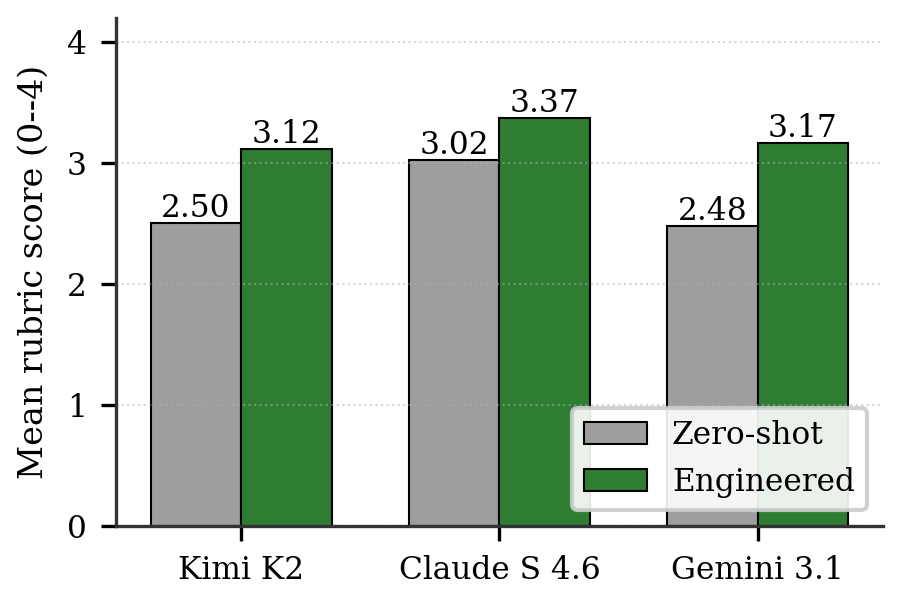
\includegraphics[width=\columnwidth]{figures/fig_cross_model.png}
\caption{Mean rubric score (0--4) per vendor in zero shot and engineered conditions. $n = 200$ prompts per cell.}
\label{fig:vendors}
\end{figure}

\begin{table}[t]
\centering
\caption{Cross vendor effect of the engineered prompt. $n = 200$ prompts per vendor.}
\label{tab:vendors}
\footnotesize
\begin{tabular}{lrrrrr}
\toprule
Vendor & zero & eng & $\Delta$ & d & $\Delta$succ \\
\midrule
Kimi K2 & 2.51 & 3.12 & 0.61 & 0.70 & +23 pp \\
Claude Sonnet 4.6 & 3.03 & 3.37 & 0.35 & 0.59 & +14 pp \\
Gemini 3.1 Pro & 2.48 & 3.17 & 0.69 & 0.80 & +24 pp \\
\bottomrule
\end{tabular}
\end{table}

Pairwise Cohen's $\kappa$ between the three vendors on the binary success label is between 0.39 and 0.43 (Fig.~\ref{fig:kappa}), which counts as moderate agreement on the Landis and Koch scale \cite{landis1977kappa}. Vendors agree on the easy and hard prompts but split on the boundary cases.

\begin{figure}[t]
\centering
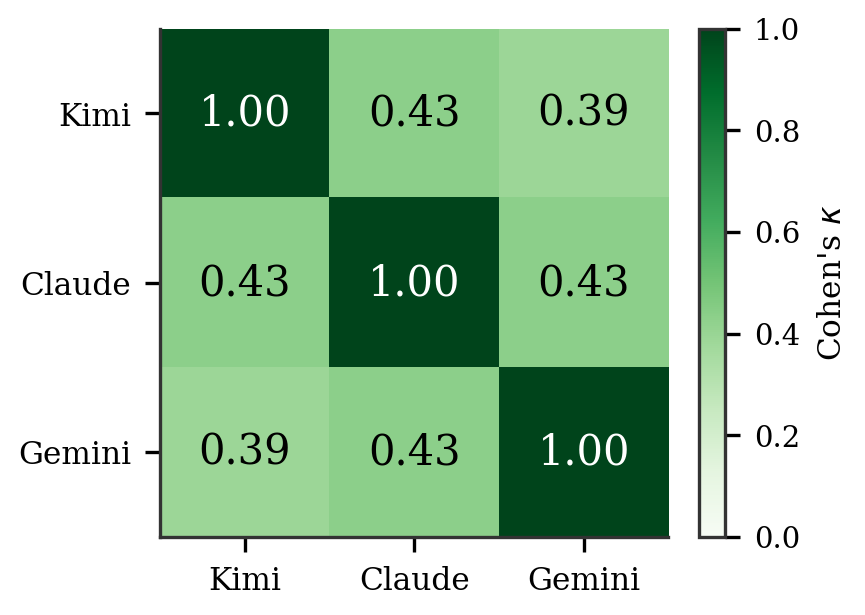
\includegraphics[width=\columnwidth]{figures/fig_kappa_heatmap.png}
\caption{Pairwise Cohen's $\kappa$ between the three vendors on the binary success label.}
\label{fig:kappa}
\end{figure}

\subsection{Manual validation of the success label}\label{sec:validation}
We drew a stratified random sample of 200 conversations and manually re labeled the first 50 against the protocol document. Cohen's $\kappa$ between the manual label and the auto label is $0.834$, with 92.0\% raw agreement and four disagreements. Under Landis and Koch this is almost perfect agreement \cite{landis1977kappa}. The four disagreements are borderline conversations where code is present but answers a related but different problem from what the user asked; the auto labeler is conservative on those.

\subsection{Language subgroups}
Table~\ref{tab:lang} reports per language ROC-AUC for the eighteen languages with at least 25 conversations. The model is most accurate on CSS, Python, and Assembly (AUC above 0.70). It performs at chance on Shell, Batchfile, and C\#, which have small sample sizes and more variable conversation styles.

\begin{table}[t]
\centering
\caption{Per language ROC-AUC, restricted to languages with $n \geq 25$.}
\label{tab:lang}
\footnotesize
\begin{tabular}{lrrr}
\toprule
Language & $n$ & success \% & ROC-AUC \\
\midrule
CSS & 1{,}313 & 73.1 & 0.809 \\
Python & 703 & 53.8 & 0.716 \\
Assembly & 25 & 72.0 & 0.700 \\
C & 136 & 63.2 & 0.668 \\
Go & 110 & 62.7 & 0.668 \\
Jupyter Notebook & 270 & 40.0 & 0.667 \\
JavaScript & 345 & 70.7 & 0.639 \\
Rust & 63 & 73.0 & 0.623 \\
TypeScript & 652 & 69.9 & 0.622 \\
Java & 163 & 68.7 & 0.620 \\
HTML & 329 & 51.4 & 0.602 \\
C++ & 186 & 50.5 & 0.579 \\
Dockerfile & 72 & 47.2 & 0.555 \\
Kotlin & 38 & 78.9 & 0.550 \\
Ruby & 26 & 73.1 & 0.500 \\
C\# & 100 & 64.0 & 0.481 \\
Batchfile & 67 & 71.6 & 0.346 \\
Shell & 30 & 70.0 & 0.315 \\
\bottomrule
\end{tabular}
\end{table}

\subsection{Temporal stability}
Fig.~\ref{fig:temporal} plots per snapshot odds ratios for the two headline behavioral features against the snapshot date. The output format effect is positive in every snapshot with $n \geq 200$, with point estimates between 1.33 and 3.62. The refinement turns effect on the per snapshot fit is below 1.0 in every snapshot, which appears to contradict the headline finding from the joint model. The two are not in conflict: the per snapshot fit does not separate refinement from correction cycles, so it confounds the two. The full model controls for correction cycles and recovers the positive refinement effect.

\begin{figure}[t]
\centering
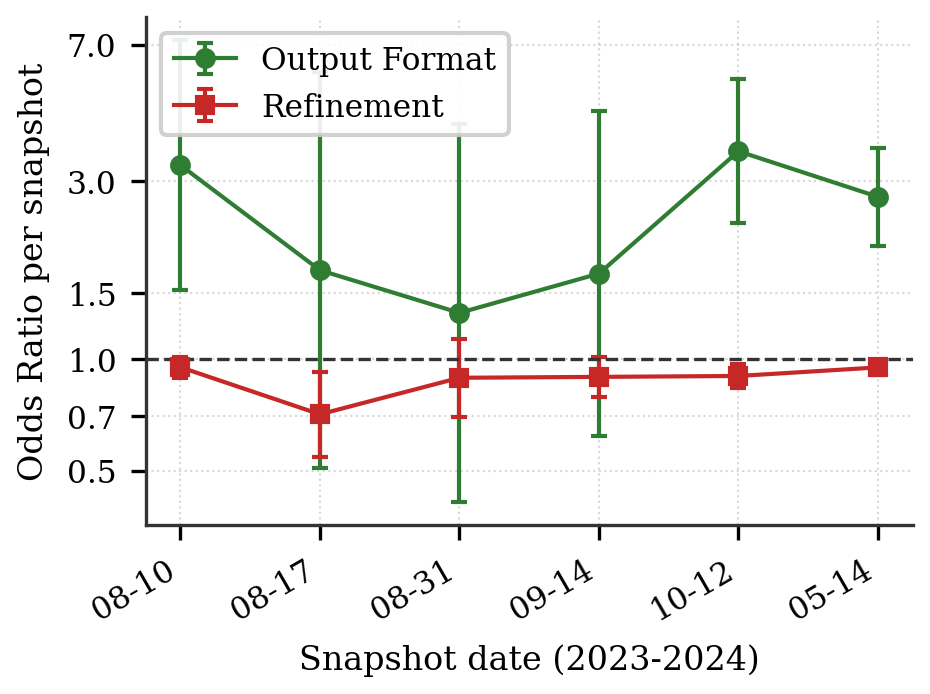
\includegraphics[width=\columnwidth]{figures/fig_temporal_drift.png}
\caption{Per snapshot odds ratios for output format and refinement turns on a log axis. Error bars are 95\% Wald CIs. Snapshots with $n < 200$ are excluded.}
\label{fig:temporal}
\end{figure}

\section{Discussion}\label{sec:discussion}
\subsection{Practical guidance for developers}
The fitted model gives a short evidence based checklist. First, add an output format instruction. A trailing ``return JSON'' or ``respond in markdown with fenced code'' alone raises the odds of a useful answer by 75\% in our data. Second, expect to refine. Each refinement turn adds 19\% to the odds of success, provided the conversation does not contain explicit corrective feedback. Refinement is part of the workflow, not a sign of trouble. Third, do not use a bare role prompt. ``You are a Python expert'' on its own slightly hurts. Combine it with an output format and the joint odds rise by a factor of about five. Fourth, keep the first prompt short and specific. Long prompts and growing prompts both correlate with worse outcomes, which probably reflects underspecified intent.

\subsection{A worked example of the role $\times$ format interaction}
Consider two prompts a developer might write for the same task. Prompt A reads, ``You are a Python expert. Help me sort a list.'' Role is present and output format is absent. The fitted joint odds factor on these two terms is $0.65 \cdot 1.0 \cdot 1.0 = 0.65$. Prompt B reads, ``You are a Python expert. Sort the list and return only valid Python code in a fenced block.'' Role and output format are both present. The joint odds factor is $0.65 \cdot 1.75 \cdot 5.28 \approx 6.0$, which is roughly nine times higher than Prompt A. The interaction term carries most of that lift. The lesson is that role instructions are not free: they need a concrete output anchor.

\subsection{Why the role main effect is negative}
A first reading of the negative role coefficient might suggest role prompting is harmful. The interaction analysis tells a different story. Role on its own correlates with vague exploratory questions, which fail more often. Role combined with an explicit output format correlates with developers who know what they want and encode it precisely. The negative main effect is therefore a confounder of user intent rather than a property of role prompting itself.

\subsection{Why refinement is positive in the joint model}
Earlier descriptive studies treat refinement as a sign of trouble. In the joint model refinement is positive once correction cycles are included as a separate covariate. Correction cycles capture the bad refinement: a wrong answer that the user must repair. Pure refinement covers clarification, follow up, and scope expansion, which is positive. Treating refinement as one variable conflates two opposing effects.

\subsection{Threats to validity}
The success label is a textual heuristic. We cannot run the code at scale, so a conversation may be labeled success even when the produced code is wrong but the user said nothing. The manual validation puts $\kappa$ at 0.83, which is strong, but the four disagreements are conservative misses; the auto labeler may slightly under count successes. The study is observational, not causal. Skilled developers may both write better prompts and choose easier tasks, and we cannot rule that out. We control for repository language, source type, snapshot, and ChatGPT model variant, but unobserved confounders such as developer experience are not in the data. We therefore frame every claim as an association after adjustment, not as a causal effect of adding a feature to a prompt. DevGPT contains conversations that the developer chose to share publicly; selection bias toward funny or dramatic conversations is a known feature of the corpus. The dataset is also English heavy and skews toward web languages such as CSS, JavaScript, and TypeScript. The cross vendor study uses a rubric judge that is itself an LLM. We mitigate by reporting effect sizes (Cohen's d) alongside p values and by using inter vendor $\kappa$ as a sanity check, but a study with human raters would strengthen the cross vendor piece.

\section{Reproducibility}\label{sec:repro}
The full pipeline is reproducible from a single command, \texttt{python main.py}, on the project repository. Inputs are the public DevGPT v10 release \cite{xiao2023devgpt}; outputs are the parquet files and JSON artifacts under \texttt{results/}.

\textbf{Software stack.} Python 3.12, \texttt{scikit-learn} 1.4, \texttt{statsmodels} 0.14, \texttt{pandas} 2.2, \texttt{numpy} 1.26, \texttt{matplotlib} 3.10, all pinned in \texttt{requirements.txt}. The random seed is fixed at 42 for every fit, fold, and resample.

\textbf{Pipeline scripts.} Each analytical step is a self contained Python script that reads only the parquet feature matrix and the labels (never the raw text) and emits a JSON or parquet artifact under \texttt{results/}:

\begin{lstlisting}
run_baselines.py        -> baselines.json
run_ablation.py         -> ablation.json
run_temporal_drift.py   -> temporal_drift.json
run_interactions.py     -> interactions.json
run_validation_kappa.py -> validation_kappa.json
multi_model_study.py    -> multi_model/
                           multi_model_study.json
\end{lstlisting}

\noindent The artifacts can be regenerated without re-fetching the corpus.

\textbf{Tables and figures.} Every table number in this paper is sourced from a CSV under \texttt{results/paper/} and every figure is generated by \texttt{make\_figures.py} (shipped with the paper bundle), which reads the same JSON and parquet artifacts. No number in the paper is typed by hand.

\textbf{Companion website.} An interactive companion at the project URL streams the cross vendor study live: a developer types a coding prompt, three vendors race in parallel, and a Claude Haiku judge grades each output against the same rubric used in the offline study. The site reads the same coefficient and ablation files referenced in this paper.

\section{Limitations}\label{sec:limitations}
The dataset window stops at May 2024, so newer ChatGPT versions are not represented. The feature set is structural and behavioral; semantic content of prompts is not modeled. A larger sample of human labeled conversations would tighten the validation $\kappa$, and a fully blinded two reviewer protocol would let us report inter human agreement separately from human against auto agreement. The interaction analysis pre registered four pairs out of a much larger set of possible two way terms; an exploratory screen with multiple comparison correction is left for future work. The success label is a textual heuristic and the study is observational rather than causal, so every claim is framed as an association after adjustment. DevGPT contains conversations the developer chose to share publicly, which introduces selection bias. The corpus is also English heavy and skews toward web languages such as CSS, JavaScript, and TypeScript, which limits external validity. The cross vendor study uses a rubric judge that is itself an LLM; we mitigate by reporting effect sizes alongside p values and by using inter vendor $\kappa$ as a sanity check, but a study with human raters would strengthen the cross vendor piece.

\section{Conclusion}\label{sec:conclusion}
We mined eleven structural and behavioral prompt features from 6{,}413 real developer ChatGPT conversations, fit a balanced logistic regression with five fold stratified cross validation, and reached ROC-AUC 0.799. Three findings carry the story. An explicit output format instruction raises the odds of a successful conversation by 75\%. Role instructions hurt on their own but help by a factor of about five when combined with an output format. The engineered prompt effect generalizes across three independent LLMs with success rates rising 14 to 24 percentage points. Feature group ablation, pre registered interactions, manual validation at $\kappa = 0.834$, per snapshot stability, and a cross vendor replication all point in the same direction. The structural prompt features carry roughly three times the predictive load of language, source type, model variant, and snapshot date combined.

\subsection{Future work}
Four directions extend this study. First, a fully blinded two reviewer human re labeling pass on a larger sample (n = 500) would let us report human against human $\kappa$ separately from human against auto $\kappa$, tightening the validation argument. Second, a causal study using natural experiments inside the DevGPT timeline, such as the GPT-3.5 to GPT-4 cutover, would move the work from association to intervention. Third, an extension to non English developer corpora and to languages outside the JavaScript and Python clusters would test external validity. Fourth, a fine grained interaction screen with Bonferroni or Benjamini-Hochberg correction over all $\binom{11}{2}$ two way terms would expose any compounding effects we missed by pre registering only four pairs.

\begin{thebibliography}{99}

\bibitem{empirical2024chatgpt}
T.\ Mohamed et al., ``An Empirical Study on Developers' Shared Conversations with ChatGPT in GitHub PRs and Issues,'' \emph{Empirical Software Engineering}, Springer, 2024.

\bibitem{wu2024promptpatterns}
Y.\ Wu et al., ``ChatGPT Chats Decoded: Uncovering Prompt Patterns for Superior Solutions in Software Development,'' \emph{ACM Conf.\ Proc.}, 2024.

\bibitem{sn2025codereview}
``Usage of Large Language Models for Code Generation Tasks: A Review,'' \emph{SN Computer Science}, Springer, 2025.

\bibitem{icsme2025prompting}
``Prompting Matters: Assessing the Effect of Prompting Techniques on LLM Generated Class Code,'' \emph{Proc.\ IEEE ICSME}, 2025.

\bibitem{elsevier2025promptengineering}
``Unleashing the Potential of Prompt Engineering for Large Language Models,'' \emph{ScienceDirect}, Elsevier, 2025.

\bibitem{xiao2023devgpt}
Z.\ Xiao et al., ``DevGPT: Studying Developer ChatGPT Conversations,'' arXiv:2309.03914, 2023.

\bibitem{acm2023security}
``Large Language Models for Code: Security Hardening and Adversarial Testing,'' \emph{ACM Digital Library}, 2023.

\bibitem{ye2025promptalchemy}
Y.\ Ye et al., ``Prompt Alchemy: Automatic Prompt Refinement for Enhancing Code Generation,'' arXiv:2503.11085, 2025.

\bibitem{schmidt2023promptcatalog}
D.\ C.\ Schmidt et al., ``A Prompt Pattern Catalog to Enhance Prompt Engineering,'' \emph{Pattern Languages of Programs (PLoP)}, 2023.

\bibitem{liu2023improvingchatgpt}
L.\ Liu et al., ``Improving ChatGPT Prompt for Code Generation,'' arXiv:2305.08360, 2023.

\bibitem{secure2024prompting}
``Prompting Techniques for Secure Code Generation: A Systematic Investigation,'' arXiv:2407.07064, 2024.

\bibitem{frontiers2024education}
``Prompt Engineering as a Next Generation Skill,'' \emph{Frontiers in Education}, 2024.

\bibitem{landis1977kappa}
J.\ R.\ Landis and G.\ G.\ Koch, ``The measurement of observer agreement for categorical data,'' \emph{Biometrics}, vol.~33, no.~1, pp.~159--174, 1977.

\bibitem{pedregosa2011sklearn}
F.\ Pedregosa et al., ``Scikit-learn: Machine Learning in Python,'' \emph{Journal of Machine Learning Research}, vol.~12, pp.~2825--2830, 2011.

\bibitem{seabold2010statsmodels}
S.\ Seabold and J.\ Perktold, ``Statsmodels: Econometric and Statistical Modeling with Python,'' \emph{Proc.\ 9th Python in Science Conf.}, 2010.

\end{thebibliography}
\end{document}
